% This section uses TikZ for the decision figure. Ensure the preamble includes: \usepackage{tikz}

\section{Comparing the Main Generative Paradigms}

We have now studied four major families of generative models in this chapter:
variational latent-variable models, adversarial models, exact invertible models, and diffusion models.
At this point the main pedagogical task is no longer definition but judgment.
A student who has understood the previous sections should be able to answer a more difficult question than ``what is a VAE?'' or ``what is a diffusion model?''
The real question is:

\begin{quote}
for a given modeling goal, which generative paradigm is structurally appropriate, which tradeoffs does it make, and which claims about it are mathematical, empirical, or merely conventional?
\end{quote}

This section therefore compares the main paradigms along a fixed set of dimensions:
objective, tractability, latent inference, sample quality, controllability, training stability, and sampling cost.
The goal is not to declare a single winner.
The goal is to learn how to choose.

\subsection*{The comparison axes}

A comparative section is only useful if the axes of comparison are made explicit.
For this chapter, the most informative axes are the following.

\paragraph{Objective.}
What quantity is optimized during training?
Examples include a variational lower bound, an adversarial game objective, exact log-likelihood, or a denoising-based variational surrogate.

\paragraph{Tractability.}
Can one evaluate or optimize the training objective exactly, approximately, or only indirectly?
This includes tractable likelihood evaluation, tractable posterior inference, and tractable gradients.

\paragraph{Latent inference.}
Does the model provide a natural map from data back to hidden variables?
In VAEs this is built in through an approximate posterior.
In flows it is exact by inversion.
In GANs it is not canonical unless one adds an encoder.
In diffusion models the internal noise states are useful computational variables, but they do not usually play the same role as a single global latent code.

\paragraph{Sample quality.}
How realistic are generated samples in practice?
This is mostly an empirical question rather than a theorem.
The answer depends strongly on architecture, dataset, and evaluation metric.

\paragraph{Controllability.}
How easily can one steer generation through labels, prompts, latent editing, or conditional structure?
The answer depends both on the family and on how conditioning is implemented.

\paragraph{Training stability.}
Does optimization behave like a single-objective problem, or like a fragile game or long iterative chain?
Again, this is partly mathematical and partly practical.

\paragraph{Sampling cost.}
Once trained, how expensive is sampling?
A model may be elegant statistically but slow operationally, or fast operationally but hard to train.

\subsection*{Family-by-family comparison}

We now compare the main families from earlier sections using these axes.
The important point is not that each family has one permanent rank, but that each one embodies a different answer to the central generative-modeling problem.

\paragraph{Variational autoencoders and related latent-variable models.}
The objective is a variational lower bound on $\log p_\theta(x)$.
Likelihood training is therefore principled, but only indirect when the posterior is intractable.
A major strength is that latent inference is built into the formulation through $q_\phi(z\mid x)$.
This makes VAEs natural when one wants compressed latent descriptions, interpolation, or amortized inference.
Their traditional weakness is that sample sharpness may lag behind the best adversarial or diffusion systems unless the decoder family and training scheme are very strong.
Sampling is fast once the latent code is drawn, but the learned latent space may mix semantically useful directions with nuisance structure.

\paragraph{Adversarial models.}
The objective is a minimax game rather than a direct likelihood objective.
This can align well with perceptual realism, which is why GANs historically became important for high-fidelity image generation.
However, there is no tractable likelihood in the standard formulation, and latent inference is not canonical unless one explicitly adds an inverse map.
Sampling is typically fast because generation is one forward pass through the generator.
The main difficulty is instability: the generator and discriminator co-evolve, so gradients can become uninformative or oscillatory.
Thus GANs are attractive when one-shot high-quality synthesis matters more than density evaluation or stable latent inference.

\paragraph{Normalizing flows.}
The objective is exact log-likelihood under an invertible change of variables.
This is mathematically clean: likelihood evaluation is exact, sampling is exact, and latent inference is exact by inversion.
The main price is architectural constraint.
Because each layer must remain invertible and its Jacobian determinant must be tractable, one often sacrifices some modeling freedom.
Flows are therefore especially appealing when exact densities, exact inverses, or principled likelihood-based comparison matter.
They are less compelling when the most important criterion is best-in-class sample quality under minimal architectural restriction.

\paragraph{Diffusion models.}
The objective is usually implemented as a denoising or noise-prediction loss derived from a variational formulation.
Training is typically much more stable than adversarial training because it reduces generation to supervised prediction over corrupted inputs.
In modern practice, diffusion models often provide very strong sample quality and good conditioning behavior.
Their main cost is sampling: naive generation requires many reverse steps.
Their internal variables are useful as a sequence of refinement states, but not always as a single semantically interpretable latent code.
Thus diffusion is attractive when quality and controllability matter more than one-pass generation speed.

\subsection*{A structured summary table}

The comparison in prose is easier to use once condensed into a single reference table.
Table~\ref{tab:gencompare} should be read as a comparative guide rather than as a ranking.
Words such as ``strong'' or ``weak'' are intentionally relative and should be interpreted as broad patterns across standard versions of each family.

\begin{table}[h]
\centering
\scriptsize
\renewcommand{\arraystretch}{1.2}
\resizebox{\textwidth}{!}{%
\begin{tabular}{|p{2.1cm}|p{2.7cm}|p{1.8cm}|p{1.8cm}|p{1.7cm}|p{1.9cm}|p{1.9cm}|p{1.8cm}|}
\hline
\textbf{Family} & \textbf{Objective} & \textbf{Tractable likelihood} & \textbf{Latent inference} & \textbf{Sample quality} & \textbf{Controllability} & \textbf{Training stability} & \textbf{Sampling cost} \\
\hline
VAE / latent-variable & ELBO or related variational objective & Approximate & Approximate posterior available & Often moderate to strong, depends on decoder & Good when latent structure is well designed & Usually good & Low after training \\
\hline
GAN & Adversarial minimax game & No, not in standard form & Not canonical without added encoder & Often very high in domains where GANs work well & Can be good conditionally, but latent control may be fragile & Often difficult & Very low \\
\hline
Flow & Exact log-likelihood by change of variables & Yes, exact & Yes, exact by inversion & Often good but constrained by invertibility requirements & Good when conditioning is built into the transform & Usually good to moderate & Low to moderate \\
\hline
Diffusion & Variational denoising / noise-prediction objective & Bound or surrogate; exact likelihood usually not the main practical interface & Reverse refinement states rather than a simple global code & Often very high in modern practice & Often strong, especially with conditional guidance & Usually good & High unless accelerated \\
\hline
\end{tabular}%
}
\caption{A comparative summary of the main generative paradigms studied in this chapter.}
\label{tab:gencompare}
\end{table}

\subsection*{Which model family for which goal?}

A table is compact, but a decision figure is better for judgment.
Figure~\ref{fig:gengoals} gives a simple decision-oriented map.
It is deliberately schematic.
Real model choice depends on domain, scale, compute budget, and engineering maturity.
Still, this diagram captures the structural logic of the comparison.

\begin{figure}[h]
\centering
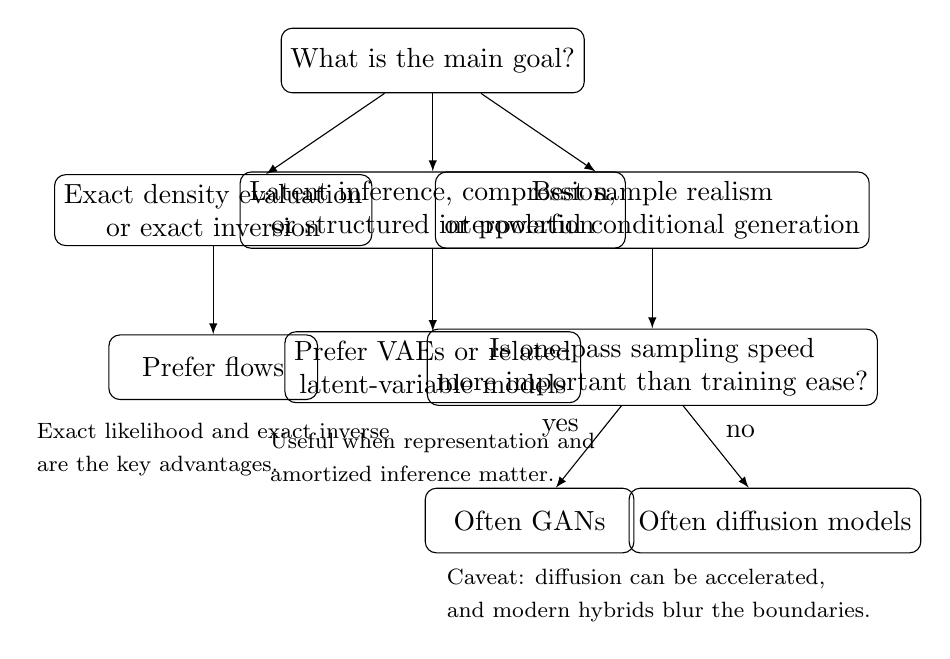
\begin{tikzpicture}[x=0.82cm,y=0.95cm,>=latex]
    \tikzstyle{box}=[draw,rounded corners,align=center,minimum width=2.65cm,minimum height=0.82cm]
    \node[box] (start) at (0,0) {What is the main goal?};
    \node[box] (likelihood) at (-3.4,-2) {Exact density evaluation\\or exact inversion};
    \node[box] (latent) at (0,-2) {Latent inference, compression,\\or structured interpolation};
    \node[box] (quality) at (3.4,-2) {Best sample realism\\or powerful conditional generation};

    \node[box] (flow) at (-3.4,-4.1) {Prefer flows};
    \node[box] (vae) at (0,-4.1) {Prefer VAEs or related\\latent-variable models};
    \node[box] (speed) at (3.4,-4.1) {Is one-pass sampling speed\\more important than training ease?};

    \node[box] (gan) at (1.5,-6.15) {Often GANs};
    \node[box] (diff) at (5.3,-6.15) {Often diffusion models};

    \draw[->] (start) -- (likelihood);
    \draw[->] (start) -- (latent);
    \draw[->] (start) -- (quality);
    \draw[->] (likelihood) -- (flow);
    \draw[->] (latent) -- (vae);
    \draw[->] (quality) -- (speed);
    \draw[->] (speed) -- node[above left] {yes} (gan);
    \draw[->] (speed) -- node[above right] {no} (diff);

    \node[align=left] at (-3.4,-5.2) {\footnotesize Exact likelihood and exact inverse\\\footnotesize are the key advantages.};
    \node[align=left] at (0,-5.3) {\footnotesize Useful when representation and\\\footnotesize amortized inference matter.};
    \node[align=left] at (3.5,-7.15) {\footnotesize Caveat: diffusion can be accelerated,\\\footnotesize and modern hybrids blur the boundaries.};
\end{tikzpicture}
\caption{A decision-oriented guide to the main generative-model families. This is not a theorem and not a universal ranking; it is a structured heuristic for matching modeling goals to paradigms.}
\label{fig:gengoals}
\end{figure}

\subsection*{What is mathematical, and what is empirical?}

A mature comparison should distinguish between statements that follow from the mathematical formulation and statements that come from repeated empirical experience.

\paragraph{Mathematical facts.}
Flows provide exact density evaluation and exact inversion by construction.
Standard GANs do not provide tractable likelihoods by construction.
VAEs optimize a lower bound on log-likelihood rather than log-likelihood itself.
Diffusion models implement generation through a learned reverse process and usually sample by many refinement steps.
These are structural statements.

\paragraph{Empirical patterns.}
Diffusion models often achieve very strong visual and multimodal sample quality.
GANs can provide excellent one-pass synthesis when training succeeds.
VAEs often provide useful latent spaces and stable training.
Flows often shine when likelihood and invertibility matter.
These are broad empirical regularities rather than universal laws.

\paragraph{Design-dependent conclusions.}
Controllability, semantic latent structure, and practical efficiency depend strongly on architecture and conditioning strategy.
For example, a diffusion model may be slow in its naive form but far faster after distillation.
A VAE may yield weak samples with a small decoder but much stronger samples with a more expressive decoder and improved objective.
A GAN may support meaningful editing if paired with a well-behaved latent space, but this is not guaranteed by the minimax objective alone.

\subsection*{How to choose in practice}

The comparison above can be compressed into a few practical recommendations.

\begin{itemize}
    \item Choose a flow when exact density evaluation, exact inversion, or principled likelihood-based comparison is central.
    \item Choose a VAE or related latent-variable model when one wants representation learning, amortized inference, compression, or latent-variable reasoning together with principled probabilistic structure.
    \item Choose a GAN when sample realism and one-shot synthesis dominate, and one is willing to manage adversarial instability and the lack of tractable likelihood.
    \item Choose a diffusion model when sample quality, conditional steering, and robust training matter more than raw sampling speed.
\end{itemize}

These recommendations are useful, but they should not harden into slogans.
Real systems often mix ideas.
Latent diffusion combines diffusion with latent-variable structure.
Flow matching and consistency-style methods alter the speed--quality tradeoff.
Conditional and multimodal systems increasingly borrow components across families.
Thus the right long-term lesson is not merely ``pick one box from the chart.''
The deeper lesson is to identify which modeling commitments actually matter for the task.

\subsection*{What to remember}

\begin{itemize}
    \item Different generative paradigms solve different mathematical subproblems well: likelihood, inference, realism, invertibility, or iterative refinement.
    \item No single family dominates every axis simultaneously.
    \item The most important comparison axes are objective, tractability, latent inference, controllability, stability, and sampling cost.
    \item Good model choice requires matching the paradigm to the goal rather than repeating current fashion.
\end{itemize}

\subsection*{Common confusion}

\begin{itemize}
    \item ``Best sample quality'' does not mean ``best for every task.''
    \item ``Has a latent space'' does not mean the latent variables are automatically interpretable or easy to control.
    \item ``Likelihood-based'' does not mean samples will necessarily look best perceptually.
    \item ``Fast sampling'' and ``easy training'' are different desiderata and often trade off against each other.
\end{itemize}

\subsection*{Exercises}

\begin{enumerate}
    \item You need a model for anomaly detection in which exact or at least principled density evaluation matters. Which family from this chapter is the strongest first candidate, and why?
    \item You need a model for image compression and smooth latent interpolation between examples. Compare VAEs and GANs for this goal. Which structural features of the objectives matter most?
    \item You need conditional image synthesis for an offline pipeline where sample quality matters more than generation speed. Which family is most attractive, and what cost does it incur?
    \item You need one-pass generation for an interactive system. Which family is attractive for speed, and what training risks come with that choice?
    \item Explain why exact invertibility is an advantage in some scientific settings but not automatically decisive for perceptual media generation.
    \item Give one modeling situation in which a diffusion model is a poor first choice, and justify your answer using the comparison axes from this section.
    \item Design your own decision chart for a domain such as molecules, audio, or robotics. Which axes from this section remain central, and which new axes would you add?
\end{enumerate}

\subsection*{Notes and References}

The four-way comparison in this section reflects the conceptual structure of the chapter rather than an exhaustive survey of generative modeling.
Autoregressive models are also central to modern generative AI, especially in language modeling, but the present chapter has focused on latent-variable, adversarial, invertible, and diffusion-based viewpoints because they illuminate different mathematical strategies for modeling a distribution.
For historical orientation, standard reference points include the VAE literature, classical GAN papers and their stability variants, the normalizing-flow literature, and the modern diffusion and score-based modeling literature.
A useful reading habit is to ask of every new generative paper the same questions used in this section: what objective is actually optimized, what inference problem is solved, what is tractable, and what practical cost is paid at sampling time?
